\documentclass{scrartcl}

\usepackage{url}
\usepackage{graphicx}
\usepackage{amsmath}
\usepackage{varwidth}
\usepackage[dvipsnames]{xcolor}
\usepackage{algorithm}
\usepackage{algpseudocode}
\usepackage{listings}
\lstset{
	basicstyle=\footnotesize\ttfamily,
	tabsize=4,
	showstringspaces=false,
	breaklines=true,
	prebreak={\space\hbox{\textcolor{Gray}{$\hookleftarrow$}}},
	language=C++
}
\usepackage{enumitem}

\usepackage{tikz}
\usetikzlibrary{shapes.geometric, arrows}

\tikzstyle{flowchartnode} = [rectangle, minimum height=0.8cm, text centered, text width=3cm, draw=black, font=\small]
\tikzstyle{startstop} = [flowchartnode, rounded corners=0.4cm]
\tikzstyle{process} = [flowchartnode]
\tikzstyle{io} = [flowchartnode, trapezium, trapezium left angle=70, trapezium right angle=110, text width=2cm]
\tikzstyle{decision} = [flowchartnode, diamond, aspect=2, text width=2cm]
\tikzstyle{arrow} = [thick,->,>=stealth]

\makeatletter
\@addtoreset{section}{part}
\makeatother  

\title{Worksheet 4}
\subtitle{COMP110: Principles of Computing}
\author{Ed Powley}
\date{January 2016}

\renewcommand\thepart{\Alph{part}}

\begin{document}

\maketitle

\section*{Introduction}

In this assignment, you will create two small C++ programs:
\begin{enumerate}[label=\Alph*.]
	\item A console application implementing the ``terminal hacking'' word-guessing minigame from the Fallout games;
%	\item A console application implementing the 2-player board game Connect~4;
	\item A graphical application which generates and displays the Mandelbrot fractal.
\end{enumerate}

This worksheet tests your ability to translate various program notations (pseudocode, flowcharts,
mathematics, narrative descriptions) into C++ code.

\section*{Submission instructions}

The GitHub repository at the following URL contains skeleton projects for the two parts of this worksheet.
\begin{center}
\url{https://github.com/Falmouth-Games-Academy/comp110-worksheet-4}
\end{center}
Fork this repository into your own GitHub account. To submit, create a GitHub pull request.

For the most part, this worksheet requires you to edit C++ code in the skeleton projects provided.
\textbf{Please do not rename or delete the projects or files provided, and please do not create new projects.}
This will ensure that GitHub's ``diff'' view highlights only the parts of the code that you have edited.
Creating new source and/or header files is permitted, if doing so improves the structure of your programs.

\section*{Marking}

\subsection*{Timely submission: $40\%$}

The deadline for this worksheet is \textbf{12noon, Monday 8th February 2016}.
To obtain the marks for timely submission, you must submit (as a GitHub pull request) your progress towards \textbf{both} parts of the worksheet by this time.
As with other worksheets, you may resubmit after these deadlines in order to collect extra correctness or quality marks.
This $40\%$ is awarded as long as you submit \emph{something} for each part by the deadline,
even if your submission has bugs or other issues.

\subsection*{Correctness: $30\%$}

To obtain the marks for correctness, you must submit working solutions for the following:
\begin{itemize}
\item Part~A, Sections~\ref{core-a-first}--\ref{core-a-last};
\item Part~B, Sections~\ref{core-c-first}--\ref{core-c-last}.
\end{itemize}
Note that this is a threshold: the full $30\%$ is awarded for work which is \emph{complete}
and contains \emph{no clear errors}. In particular you will not be penalised for trivial errors which do not
affect the overall functioning of your programs, nor will you receive extra credit for highly polished solutions.

\subsection*{Quality: $30\%$}

The extra quality criteria for this worksheet are as follows. All are weighted equally, so each is worth $6\%$ of the overall mark for this worksheet.
\begin{enumerate}
\item\textbf{Presentation.} Your solutions are appropriately presented in GitHub, with descriptive commit messages
	and appropriate documentation in \texttt{readme.md} files.
	You have edited the provided skeleton projects, and refrained from renaming the provided files or creating new projects.
    You have checked code into GitHub regularly whilst working on the worksheet.
\item\textbf{Code quality.} Your code is well formatted.
    Variable and function names are clear and descriptive.
    Comments are used where appropriate, and are well written.
    Your formatting, naming and commenting follow consistent conventions.
\item\textbf{Part A stretch goal.} You have submitted a working solution for Part~A, Section~\ref{stretch-a} (an improved word selection algorithm for the terminal hacking game).
%\item\textbf{Part B stretch goal.} You have submitted a working solution for Part~B, Section~\ref{stretch-b} (a rule variant for Connect~Four).
\item\textbf{Part B stretch goal.} You have submitted a working solution for Part~B, Section~\ref{stretch-c} (a generator for a fractal other than the Mandelbrot set).
\item\textbf{Sophistication.} Your solution for \textbf{either} of the stretch goals is particularly sophisticated,
	demonstrating mastery of C++ programming concepts appropriate to the task at hand.
    (N.B.: the emphasis here is on \emph{appropriate}; you will not receive extra credit for shoehorning advanced constructs into your code where a simpler solution would have sufficed.)
\end{enumerate}

\clearpage
\part{Terminal Hacking}

\begin{figure}
    \begin{center}
        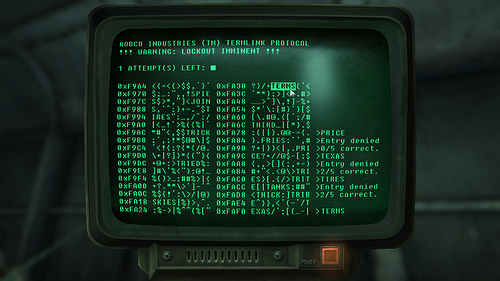
\includegraphics[width=0.8\textwidth]{fallout_terminal.jpg}
    \end{center}
    \caption{A screenshot of the hacking minigame in \emph{Fallout~4}.
    Image from \protect\url{http://fallout.wikia.com/wiki/Terminal}.}
    \label{fig:fallout_terminal}
\end{figure}

In this part, you will implement a version of the ``terminal hacking'' minigame from \emph{Fallout~4} (Bethesda, 2015); see Figure~\ref{fig:fallout_terminal}.
In this minigame you must guess a secret $n$-letter word, one of several options presented to you.
On choosing an option, you are told the \emph{likeness}: the number of letters which match the secret word (i.e.\ the same letter in the same position).
For example if the secret word is \texttt{HOUSE} and your guess is \texttt{MOUSE}, the likeness is $4$ out of $5$.
If your guess is \texttt{HOPES}, the likeness is $2$ out of $5$ (the letters \texttt{S} and \texttt{E} do not count as they are in the wrong positions).

The GitHub repository contains a project named \texttt{PartA\_TerminalHacking} for you to build upon.
This contains code to read words from a file, and choose the secret word and other words.
You will implement the rest of the game.

\section{} \label{core-a-first}

Algorithm~\ref{alg:a_likeness} takes a guessed word and the secret word, and returns the likeness score as described above.

\textbf{Implement} the algorithm as a C++ function in \texttt{TerminalHacking.cpp}, choosing appropriate data types for the parameters, return value, and any variables.

\begin{algorithm}[t]
\begin{algorithmic}
    \Procedure{GetLikeness}{guessedWord, secretWord}
        \State $\text{result} \gets 0$
        \For{$i = 0, 1, \dots, \text{secretWord.length} - 1$}
            \If{$\text{secretWord}[i] = \text{guessedWord}[i]$}
                \State increment result
            \EndIf
        \EndFor
        \State \textbf{return} result
    \EndProcedure
\end{algorithmic}
\caption{An algorithm for calculating the likeness score for the terminal hacking minigame.}
\label{alg:a_likeness}
\end{algorithm}

\section{} \label{core-a-last}

\textbf{Implement} the main loop of the game, structured
according to the flowchart shown in Figure~\ref{fig:flowchart_a}.

\begin{figure}
\begin{center}
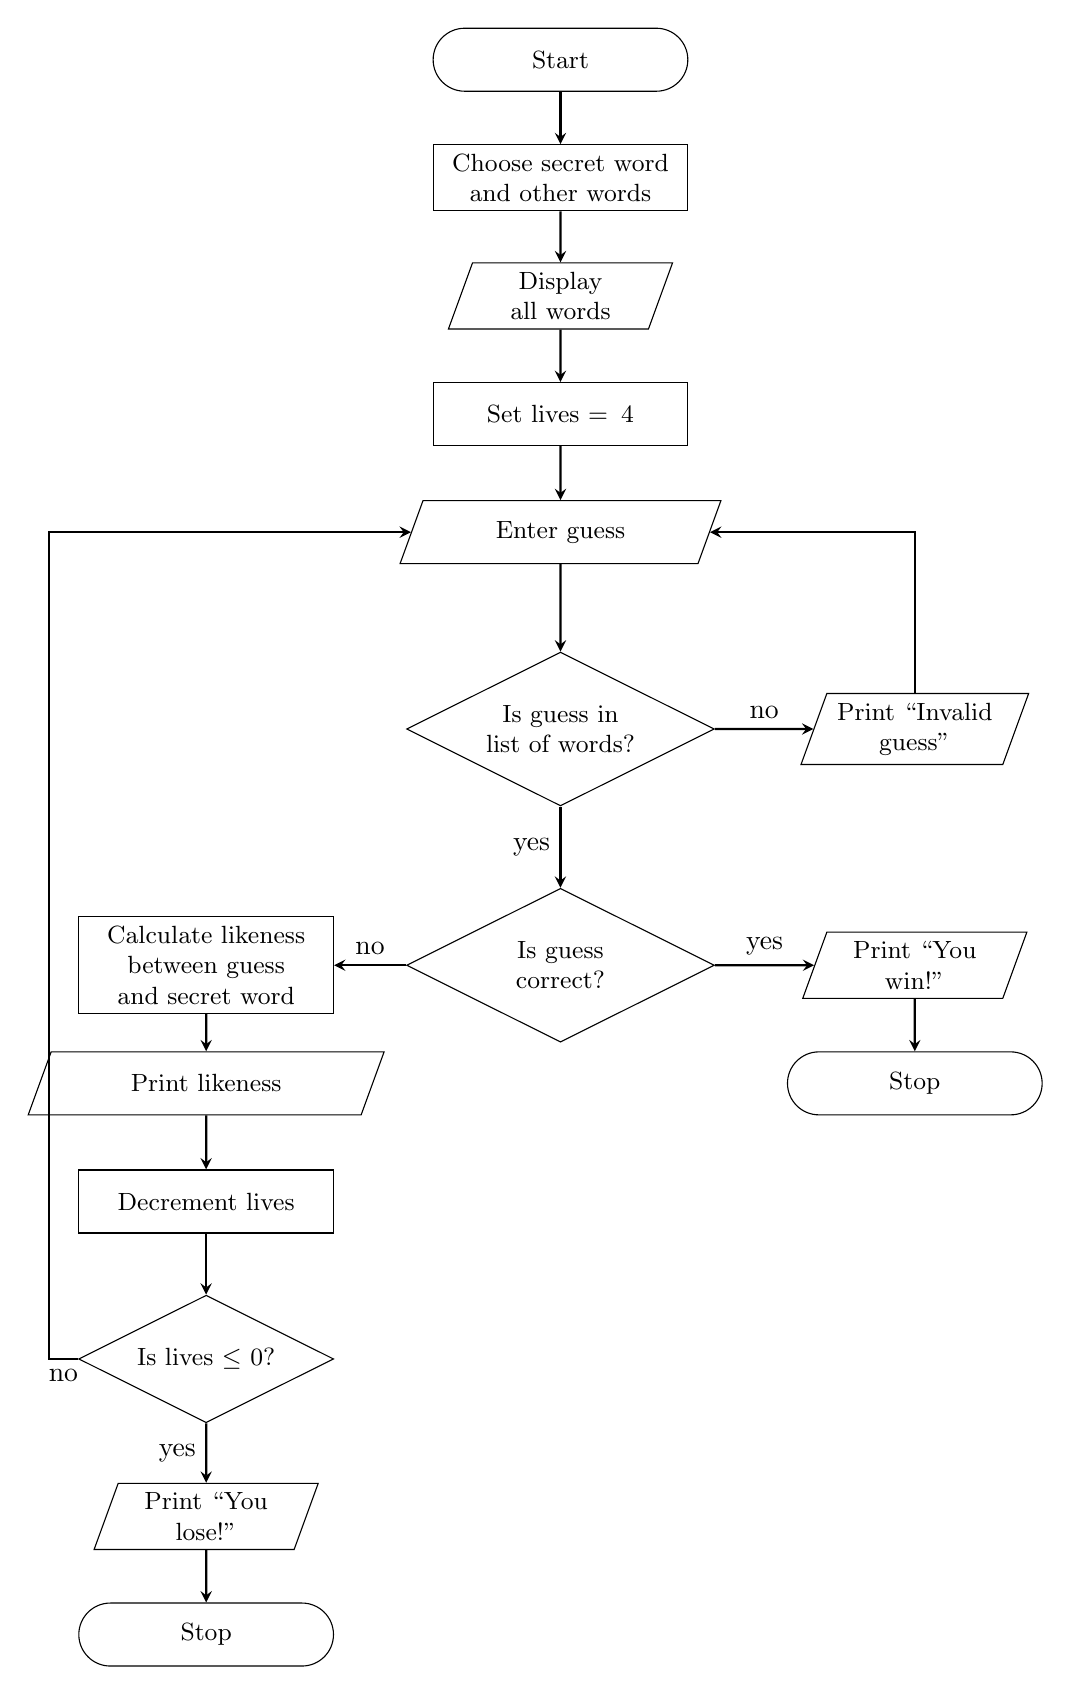
\begin{tikzpicture}[node distance=1.5cm]
\node (start) [startstop] {Start};
\node (choosewords) [process, below of=start] {Choose secret word and other words};
\node (displaywords) [io, below of=choosewords] {Display all words};
\node (initlives) [process, below of=displaywords] {Set lives $= 4$};
\node (enterguess) [io, below of=initlives] {Enter guess};
\node (isguessvalid) [decision, below of=enterguess, yshift=-1cm] {Is guess in list of words?};
\node (guessinvalid) [io, right of=isguessvalid, xshift=3cm] {Print ``Invalid guess''};
\node (isguesscorrect) [decision, below of=isguessvalid, yshift=-1.5cm] {Is guess correct?};
\node (youwin) [io, right of=isguesscorrect, xshift=3cm] {Print ``You win!''};
\node (stopwin) [startstop, below of=youwin] {Stop};
\node (calclikeness) [process, left of=isguesscorrect, xshift=-3cm] {Calculate likeness between guess and secret word};
\node (showlikeness) [io, below of=calclikeness] {Print likeness};
\node (loselife) [process, below of=showlikeness] {Decrement lives};
\node (isdead) [decision, below of=loselife, yshift=-0.5cm] {Is lives $\leq 0$?};
\node (youlose) [io, below of=isdead, yshift=-0.5cm] {Print ``You lose!''};
\node (stoplose) [startstop, below of=youlose] {Stop};
\draw [arrow] (start) -- (choosewords);
\draw [arrow] (choosewords) -- (displaywords);
\draw [arrow] (displaywords) -- (initlives);
\draw [arrow] (initlives) -- (enterguess);
\draw [arrow] (enterguess) -- (isguessvalid);
\draw [arrow] (isguessvalid) -- node[anchor=south] {no} (guessinvalid);
\draw [arrow] (guessinvalid) |- (enterguess);
\draw [arrow] (isguessvalid) -- node[anchor=east] {yes} (isguesscorrect);
\draw [arrow] (isguesscorrect) -- node[anchor=south] {yes} (youwin);
\draw [arrow] (youwin) -- (stopwin);
\draw [arrow] (isguesscorrect) -- node[anchor=south] {no} (calclikeness);
\draw [arrow] (calclikeness) -- (showlikeness);
\draw [arrow] (showlikeness) -- (loselife);
\draw [arrow] (loselife) -- (isdead);
\draw [arrow] (isdead) -- node[anchor=east] {yes} (youlose);
\draw [arrow] (youlose) -- (stoplose);
\coordinate[left of=isdead, xshift=-0.5cm] (tmp1);
\draw [arrow] (isdead) -- node[anchor=north] {no} (tmp1) |- (enterguess);
\end{tikzpicture}
\end{center}
\caption{Flowchart for the Terminal Hacking game}
\label{fig:flowchart_a}
\end{figure}

\section{Stretch goal} \label{stretch-a}

In the skeleton project, the words are chosen at random.
This may lead to instances of the game which are unsatisfying, for example where all words
have a low likeness score with respect to the secret word.

\textbf{Design} an improved word choosing algorithm.
Present your algorithm as pseudocode and/or a flowchart in your \texttt{readme.md} file on GitHub.

\textbf{Implement} your algorithm within your C++ project.


%\clearpage
%\part{Connect Four}

\begin{figure}
    \begin{center}
        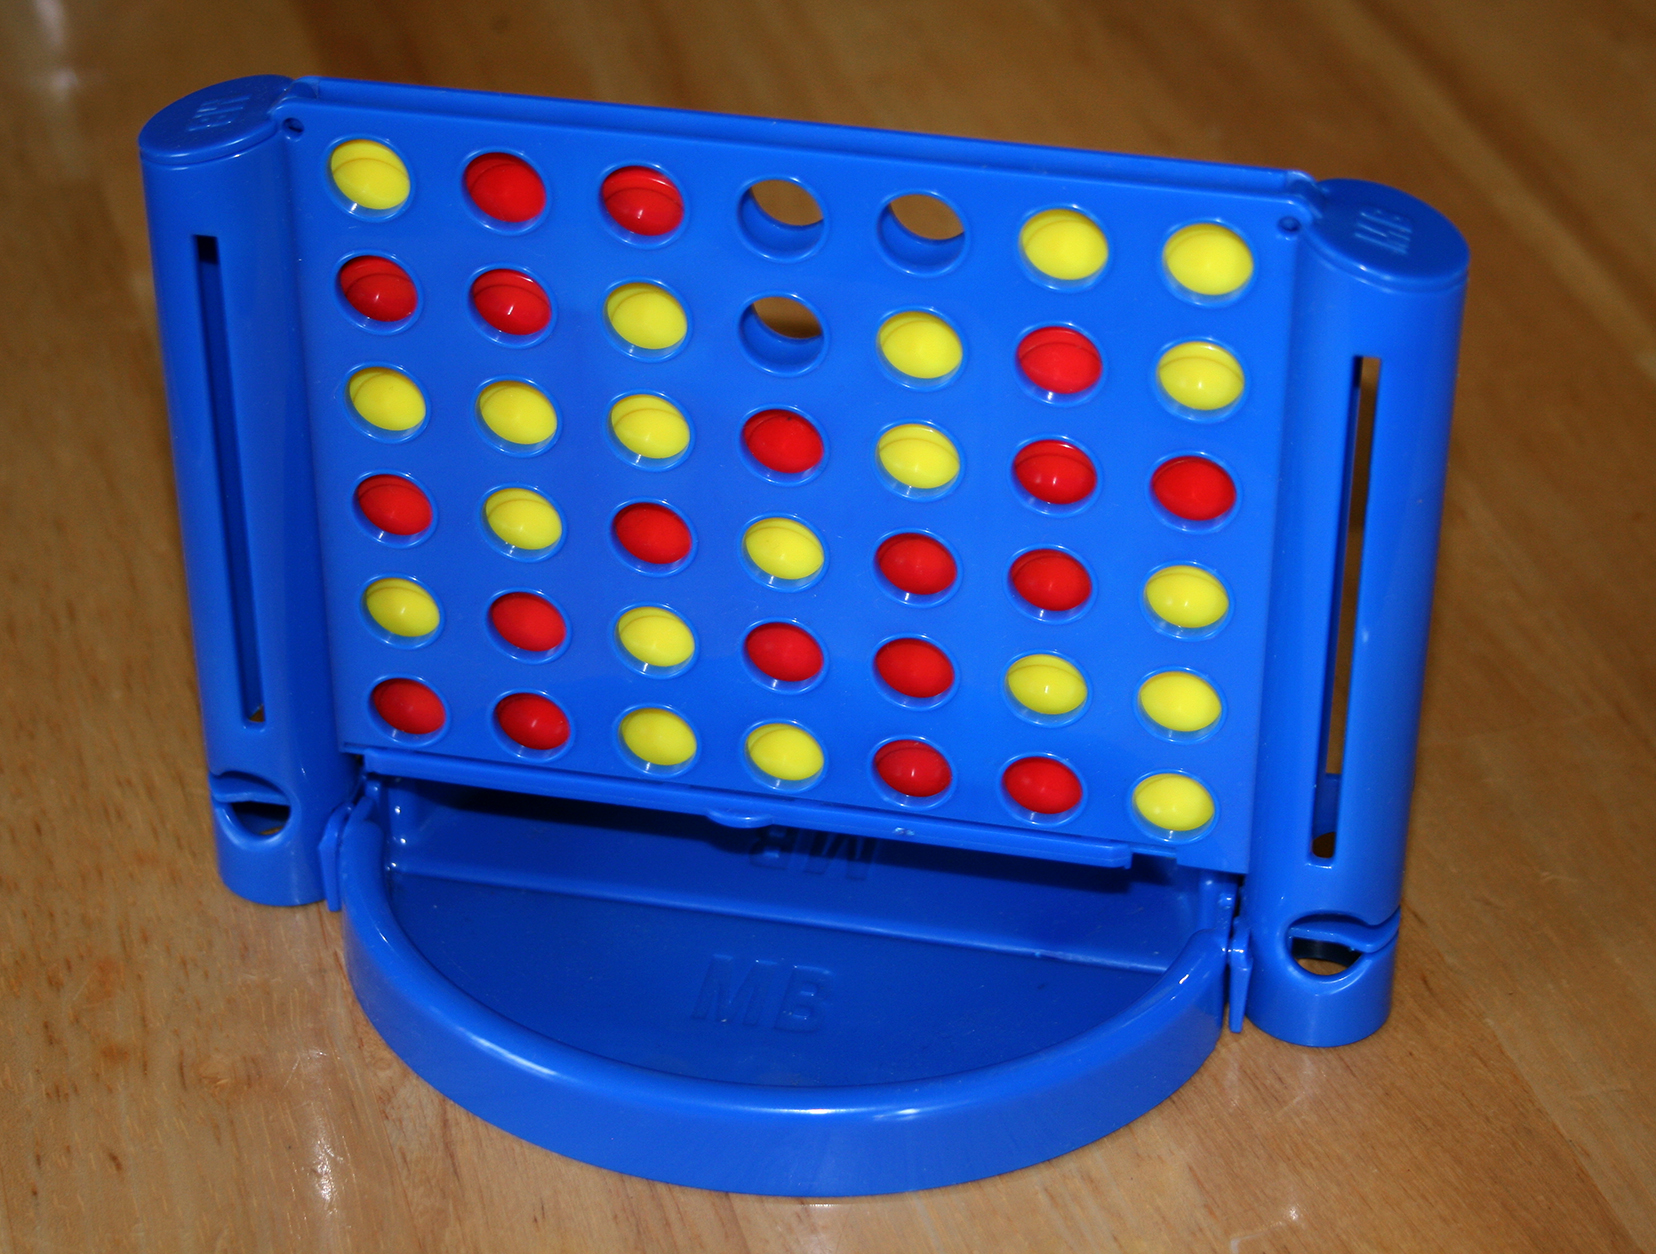
\includegraphics[width=0.6\textwidth]{connect_4.jpg}
    \end{center}
    \caption{A \emph{Connect~Four} board.
        The red player has won the game with a diagonal line starting in the lower left corner.
        Image from \protect\url{https://commons.wikimedia.org/wiki/File:Connect_Four.jpg}.}
    \label{fig:connect_4}
\end{figure}

In this part, you will implement a version of the board game \emph{Connect~Four} (Milton Bradley, 1974); see Figure~\ref{fig:connect_4}.
This is a 2-player game, in which players take turns dropping coloured counters into the top of an upright grid.
The counter falls into the lowest unoccupied space in the chosen column.
The winner is the first player to make a horizontal, vertical or diagonal line of four counters of her colour.

\section{} \label{core-b-first}

\textbf{Implement} the method \lstinline{Board::performMove}.
This method should simulate the player dropping a counter into the top of the given column \lstinline{x};
i.e.\ it should determine the lowest unoccupied square
(the largest value of \lstinline{y} such that \lstinline{getSquare(x, y) == 0})
and place the player's counter there.
It should return \lstinline{false} if the column is full, otherwise it should return \lstinline{true}.

\section{}

Algorithm~\ref{alg:b_checkline} checks for a single row of $4$ counters on the board.
The coordinates $s_x, s_y$ give the starting point of the line,
and $d_x, d_y$ (which should both be $-1$, $0$ or $+1$) give the direction.
For example $s_x=1, s_y=2, d_x=1, d_y=0$ checks the line starting at position $(1,2)$
and moving horizontally to the right.

\textbf{Implement} this algorithm as the method \lstinline{Board::checkLine} in \texttt{Board.cpp}.

\begin{algorithm}[t]
\begin{algorithmic}
    \Procedure{CheckLine}{board, $s_x$, $s_y$, $d_x$, $d_y$}
        \If{$\text{board}[s_x, s_y]$ is empty}
            \State \textbf{return} false
        \EndIf
        \For{$i = 1, 2, 3$}
            \State $t_x \gets s_x + d_x \times i$
            \State $t_y \gets s_y + d_y \times i$
            \If{$t_x, t_y$ is outside the bounds of the board}
                \State \textbf{return} 0
            \ElsIf{$\text{board}[t_x, t_y] \neq \text{board}[s_x, s_y]$}
                \State \textbf{return} 0
            \EndIf
        \EndFor
        \State \textbf{return} $\text{board}[s_x, s_y]$
    \EndProcedure
\end{algorithmic}
\caption{An algorithm for checking the presence of a single line on the Connect~Four board.}
\label{alg:b_checkline}
\end{algorithm}

\section{}

Given the above function, it is possible to check the entire board for a winning line as follows.
Loop through each square on the board.
For each square, use $\Call{CheckLine}$ to check for the following four lines:
\begin{itemize}
\item A horizontal line ($d_x=1, d_y=0$)
\item A vertical line ($d_x=1, d_y=0$)
\item A diagonal line ($d_x=1, d_y=1$)
\item A diagonal line in the other direction ($d_x=1, d_y=-1$)
\end{itemize}
If $\Call{CheckLine}$ returns true for any of these, then the winner is the player who owns the square
currently being considered.
If $\Call{CheckLine}$ never returns true for any square on the board, then there is no winner.

\textbf{Implement} this algorithm as the method \lstinline{Board::checkWin} in \texttt{Board.cpp}.

\section{} \label{core-b-last}

\textbf{Implement} the main loop of the game, structured
according to the flowchart shown in Figure~\ref{fig:flowchart_b}.

\begin{figure}
\begin{center}
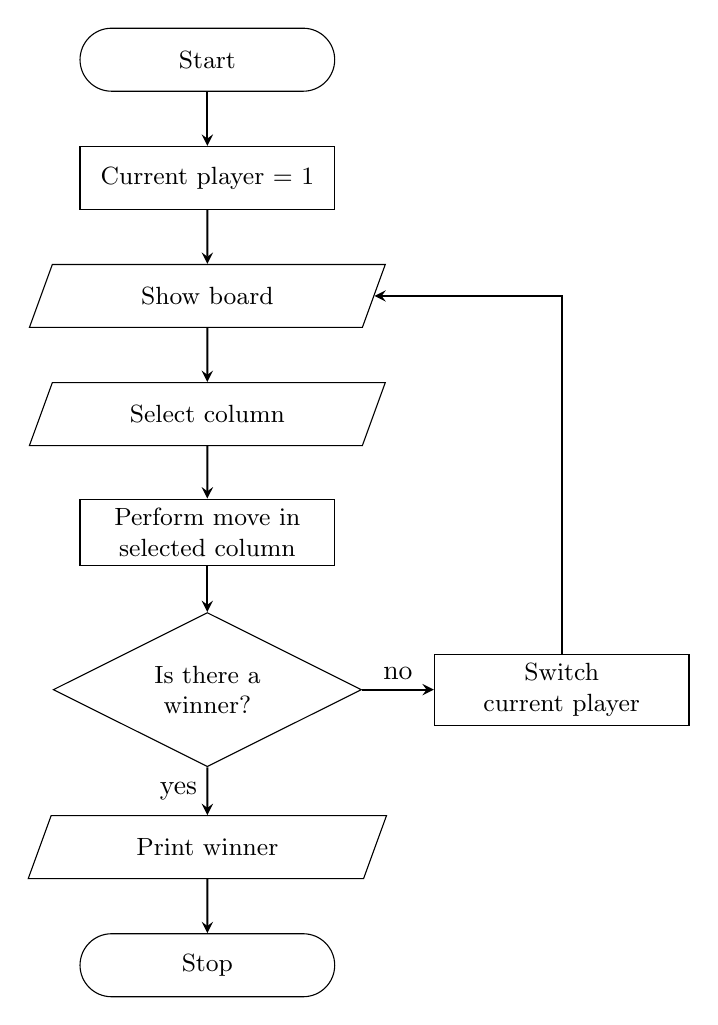
\begin{tikzpicture}[node distance=1.5cm]
\node (start) [startstop] {Start};
\node (init) [process, below of=start] {Current player = 1};
\node (displayboard) [io, below of=init] {Show board};
\node (entermove) [io, below of=displayboard] {Select column};
\node (domove) [process, below of=entermove] {Perform move in selected column};
\node (iswin) [decision, below of=domove, yshift=-0.5cm] {Is there a winner?};
\node (youwin) [io, below of=iswin, yshift=-0.5cm] {Print winner};
\node (stopwin) [startstop, below of=youwin] {Stop};
\node (switchplayer) [process, right of=iswin, xshift=3cm] {Switch \mbox{current} player};
\draw [arrow] (start) -- (init);
\draw [arrow] (init) -- (displayboard);
\draw [arrow] (displayboard) -- (entermove);
\draw [arrow] (entermove) -- (domove);
\draw [arrow] (domove) -- (iswin);
\draw [arrow] (iswin) -- node[anchor=east] {yes} (youwin);
\draw [arrow] (youwin) -- (stopwin);
\draw [arrow] (iswin) -- node[anchor=south] {no} (switchplayer);
\draw [arrow] (switchplayer) |- (displayboard);
\end{tikzpicture}
\end{center}
\caption{Flowchart for the Connect 4 game.}
\label{fig:flowchart_b}
\end{figure}

\section{Stretch goal} \label{stretch-b}

The Wikipedia page for Connect~Four lists several variants of the game with modified rules (\url{https://en.wikipedia.org/wiki/Connect_Four#Rule_variations}).

\textbf{Implement} a new program, based on your Connect~Four program, implementing a rule variant of your choice.


\clearpage
\part{Mandelbrot}

\begin{figure}
    \begin{center}
        
\includegraphics[width=0.6\textwidth]{mandelbrot.png}
    \end{center}
    \caption{The Mandelbrot set fractal.}
    \label{fig:mandelbrot}
\end{figure}

In this part, you will use the CImg library (\url{http://cimg.eu/}) to write a program to generate and display the \emph{Mandelbrot set} fractal; see Figure~\ref{fig:mandelbrot}.
This fractal colours each pixel of the image according to an iterated mathematical formula, as described below.

\section{} \label{core-c-first}

To generate an interesting fractal, the on-screen $x$ and $y$ coordinates must first be rescaled.
In the skeleton project the pixel coordinates range from $0$ to $800$,
whereas the Mandelbrot set fractal is most interesting in the region $-2 \leq x \leq 1$ and $-1.5 \leq y \leq 1.5$.

Let $p_x$ be the $x$ coordinate of the pixel. This can be remapped into the range $x_{\text{min}}$ to $x_{\text{max}}$ using the following formula:
\begin{equation*}
    x_0 = \frac{p_x}{\text{image.width}} \times \left( x_{\text{max}} - x_{\text{min}} \right) + x_{\text{min}}
\end{equation*}
The $y$ coordinate can be remapped using a similar formula.

\textbf{Implement} the above calculations for the $x$ and $y$ coordinates, at the indicated parts of \texttt{PartC\_Mandelbrot.cpp}.

\section{} \label{core-c-last}

The Mandelbrot set is based on the following sequence of numbers. Let $x_0$ and $y_0$ be the coordinates of a point in the image.
Then the sequence $x_1, y_1, x_2, y_2, x_3, y_3, \dots$ is defined\footnote{%
    If you are familiar with complex numbers, you may notice that this is equivalent to $z_{j+1} = z_j^2 + z_0$, where $z_j = x_j + y_j i$.
} recursively for $i = 0, 1, 2, 3, \dots$ by:

\begin{align*}
    x_{i+1} &= (x_i)^2 - (y_i)^2 + x_0 \\
    y_{i+1} &= (2 \times x_i \times y_i) + y_0 \\
\end{align*}

The points are coloured according to the \emph{smallest} value of $i$ for which $(x_i)^2 + (y_i)^2 \geq 4$.
If such a value of $i$ is not found after a large number of iterations (for example $i=200$), the pixel is coloured black.

\textbf{Implement} an algorithm which performs the above computation, determining the smallest value of $i$
for which $(x_i)^2 + (y_i)^2 \geq 4$ and selecting the appropriate pixel colour.
Implement the algorithm in \texttt{PartC\_Mandelbrot.cpp} so that the program generates the Mandelbrot set fractal (Figure~\ref{fig:mandelbrot}) when it is run.

\section{Stretch goal} \label{stretch-c}

Mathematicians have discovered many other fractals besides the Mandelbrot set.

\textbf{Implement} a new program, based on your Mandelbrot program,
to generate a different type of fractal which you have found online or in the academic literature.


\end{document}
